\documentclass[12pt]{article}
\usepackage[utf8]{inputenc}
\usepackage{geometry}
\geometry{letterpaper, margin=0.25in}
\usepackage{graphicx} 
\usepackage{parskip}
\usepackage{booktabs}
\usepackage{array} 
\usepackage{paralist} 
\usepackage{verbatim}
\usepackage{subfig}
\usepackage{fancyhdr}
\usepackage{sectsty}
\usepackage[shortlabels]{enumitem}

\pagestyle{fancy}
\renewcommand{\headrulewidth}{0pt} 
\lhead{}\chead{}\rhead{}
\lfoot{}\cfoot{\thepage}\rfoot{}

%%% ToC (table of contents) APPEARANCE
\usepackage[nottoc,notlof,notlot]{tocbibind} 
\usepackage[titles,subfigure]{tocloft}
\renewcommand{\cftsecfont}{\rmfamily\mdseries\upshape}
\renewcommand{\cftsecpagefont}{\rmfamily\mdseries\upshape} %

\usepackage{amsmath}
\usepackage{amssymb}
\usepackage{mathtools}
\usepackage{empheq}
\usepackage{xcolor}
\usepackage{bbm}
\usepackage{tikz}
\usepackage{pgfplots}
\usepackage{tikz-cd}
\pgfplotsset{compat=1.18}
\usetikzlibrary{intersections, decorations.markings}
\tikzset{
    marking along/.style n args={2}{
        decoration={
                markings, 
                mark=at position #1 with {\arrow{#2}}
        },
        postaction={decorate}
        },
    marking along/.default={0.5}{>}
    wavy/.style={
        decorate,decoration={coil,aspect=0}
     },
    two marks/.style n args={1}{
        decoration={
            markings,
            mark=at position 0.25 with {\arrow{#1}},
            mark=at position 0.75 with {\arrow{#1}}
         },
         postaction={decorate}
    }
}

\colorlet{mygreen}{green!50!teal}

\newcommand{\ans}[1]{\boxed{\text{#1}}}
\newcommand{\vecs}[1]{\langle #1\rangle}
\renewcommand{\hat}[1]{\widehat{#1}}

\renewcommand{\P}{\mathbb{P}}
\newcommand{\R}{\mathbb{R}}
\newcommand{\E}{\mathbb{E}}
\newcommand{\Z}{\mathbb{Z}}
\newcommand{\N}{\mathbb{N}}
\newcommand{\Q}{\mathbb{Q}}
\newcommand{\C}{\mathbb{C}}

\newcommand{\ind}{\mathbbm{1}}
\newcommand{\qed}{\quad \blacksquare}

\newcommand{\brak}[1]{\left\langle #1 \right\rangle}
\newcommand{\bra}[1]{\left\langle #1 \right\vert}
\newcommand{\ket}[1]{\left\vert #1 \right\rangle}

\newcommand{\abs}[1]{\left\vert #1 \right\vert}
\newcommand{\mfX}{\mathfrak{X}}
\newcommand{\ep}{\varepsilon}

\newcommand{\Ec}{\mathcal{E}}
\newcommand{\Nc}{\mathcal{N}}
\newcommand{\A}{\mathcal{A}}
\newcommand{\F}{\mathcal{F}}
\newcommand{\Cc}{\mathcal{C}}
\newcommand{\B}{\mathcal{B}}
\newcommand{\M}{\mathcal{M}}
\newcommand{\X}{\chi}
\renewcommand{\L}{\mathcal{L}}

\newcommand{\sub}{\subseteq}
\newcommand{\st}{\text{ s.t. }}
\newcommand{\card}{\text{card }}
\renewcommand{\div}{\vspace*{10pt}\hrule\vspace*{10pt}}
\newcommand{\surj}{\twoheadrightarrow}
\newcommand{\inj}{\hookrightarrow}
\newcommand{\biject}{\hookrightarrow \hspace{-8pt} \rightarrow}
\renewcommand{\bar}[1]{\overline{#1}}
\newcommand{\overcirc}[1]{\overset{\circ}{#1}}
\newcommand{\diam}{\text{diam }}
\newcommand{\iid}{\overset{	ext{iid}}{\sim}}

\renewcommand{\Re}{\text{Re}\,}
\renewcommand{\Im}{\text{Im}\,}
\newcommand{\Var}{\text{Var}\,}
\newcommand{\Cov}{\text{Cov}\,}

\DeclareMathOperator*{\argmax}{\arg\max}
\DeclareMathOperator*{\argmin}{\arg\min}

\newcommand{\sign}{\text{sign}\,}
\newcommand{\tr}{\text{tr}\,}


\newcommand*{\tbf}[1]{\ifmmode\mathbf{#1}\else\textbf{#1}\fi}

\usepackage{tcolorbox}
\tcbuselibrary{breakable, skins}
\tcbset{enhanced}
\newenvironment*{tbox}[2][gray]{
    \begin{tcolorbox}[
        parbox=false,
        colback=#1!5!white,
        colframe=#1!75!black,
        breakable,
        title={#2}
    ]}
    {\end{tcolorbox}}

\newenvironment*{exercise}[1][red]{
    \begin{tcolorbox}[
        parbox=false,
        colback=#1!5!white,
        colframe=#1!75!black,
        breakable
    ]}
    {\end{tcolorbox}}

\newenvironment*{proof}[1][blue]{
\begin{tcolorbox}[
    parbox=false,
    colback=#1!5!white,
    colframe=#1!75!black,
    breakable
]}
{\end{tcolorbox}}
\newenvironment*{proposition}[1][gray]{
    \begin{tcolorbox}[
        parbox=false,
        colback=#1!5!white,
        colframe=#1!75!black,
        breakable
    ]}
    {\end{tcolorbox}}

\title{APMA 1360: Midterm II Practice Exam}
\author{Milan Capoor}
\date{}

\begin{document}
\maketitle

\section{Problem 1}

\begin{enumerate}[(a)]
    \item Consider $u \in \R^n, \mu \in \R$, and $F(u, \mu) \in \R^n$. Assume $F(0,0) = 0$ and let $A := F_u(0,0)$. Which of the conditions below guarantee that we can solve the equation $F(u, \mu) = 0$ for $u$ as a function of $\mu$ near $(u,\mu) = 0$? Circle all that apply:
          \begin{itemize}
              \item \textcolor{blue}{$\boxed{\text{A is invertible}}$}
              \item $\det A = 0$
              \item All eigenvalues of $A$ have strictly negative real part
              \item $A \neq 0$
          \end{itemize}

    \item Is the following phase diagram configuration possible or not? Support your answer.

          \begin{center}
              \includegraphics[width=0.5\textwidth]{1b.png}
          \end{center}

          \color{blue}
          No. $I(\text{saddle}) = -1$ and $I(\text{attractor}) = 1$ so $I(\text{orbit}) = -1 -1 + 1 = -1$ but the index of a periodic orbit is always $1$.
          \color{black}


    \item Can the following phase diagram arise from a gradient system? Support your answer (in a few
          brief lines).

          \begin{center}
              \includegraphics[width=0.4\textwidth]{1c.png}
          \end{center}

          \color{blue}
          No. Since gradient systems have a Lyapunov functional ($V$ for $\dot u = -\nabla V(u)$), by a Lemma, the system cannot have a (nontrivial) periodic orbit.
          \color{black}

\end{enumerate}

\pagebreak

\section{Problem 2}
Compute the indices of all equilibria of the two systems
\[\begin{pmatrix}
        \dot x \\
        \dot y
    \end{pmatrix} = \begin{pmatrix}
        -x - 2y \\
        -3y
    \end{pmatrix}, \qquad \begin{pmatrix}
        \dot x \\
        \dot y
    \end{pmatrix} = \begin{pmatrix}
        -x^2 - y^2 \\
        0
    \end{pmatrix}\]

\color{blue}
First,
\[\begin{cases}
        0 = -x - 2y \\
        0 = -3y
    \end{cases} \implies \begin{cases}
        y = 0 \\
        x = 0
    \end{cases} \implies (0, 0) \text{ is only equilibrium}\]

Then,
\[J(x, y) = \begin{pmatrix}
        -1 & -2 \\
        0  & -3
    \end{pmatrix} \implies \lambda = \{-1, -3\} \implies (0, 0) \text{ attractor} \implies \boxed{I(0, 0) = 1}\]

\div

\color{red}
Similarly,
\[\begin{cases}
        0 = -x^2 - y^2 \\
        0 = 0
    \end{cases} \implies (0, 0) \text{ only equilibrium }\]
and
\[J(x, y) = \begin{pmatrix}
        -2x & -2y \\
        0   & 0
    \end{pmatrix} \implies J(0, 0) = \begin{pmatrix}
        0 & 0 \\
        0 & 0
    \end{pmatrix} \implies \text{inconclusive}\]




\color{black}


\pagebreak

\section{Problem 3}
Find a value of $a$ for which $E(u,v) = u^2+ av^2$ is a Lyapunov functional of
\begin{align*}
    \dot u & = -u -2v - 2u^3 \\
    \dot v & = -3v + u - v^3
\end{align*}

\color{blue}

\begin{align*}
    \nabla E(u, v)     & = \begin{pmatrix}
                               2u \\
                               2av
                           \end{pmatrix}                                                \\
    \brak{\nabla E, F} & = 2u(-u - 2v - 2u^3) + 2av(-3v + u - v^3)                       \\
                       & = -2u^2 - 4uv - 4u^4 - 6av^2 + 2auv - 2av^4                     \\
                       & = (2a - 4)uv - 6av^2 + \underbrace{(-2u^2 - 4u^4 - 2av^4)}_{<0} \\
\end{align*}

If $\text{sign}(u) = \text{sign}(v)$, then we need $0 < a \leq 2$ to ensure the function is negative. If $\text{sign}(u) \neq \text{sign}(v)$, then we need $a \geq 2$ to ensure the function is negative. Hence, for $\boxed{a = 2}$, $E$ is a Lyapunov functional for all $u, v$.

\color{black}


\pagebreak

\section{Problem 4}
Sketch the phase diagram and classify all equilibria of the second-order equation $\ddot u = f(u)$ where the graph of the function $-\int^u f(x)\; dx$

\begin{center}
    \includegraphics[width=0.8\textwidth]{4.png}

\end{center}


\pagebreak

\section{Problem 5}
The figure shown below contains the two nullclines of the system
\begin{align*}
    \dot x & = f(x,y) \\
    \dot y & = g(x,y)
\end{align*}

\begin{center}
    \begin{tikzpicture}
        \node at (0, 0) {\includegraphics[width=0.8\textwidth]{5.png}};
        \node[red, scale=2] at (-1, -0.25) {$\bullet$};

        \draw[->, gray] (-2, 4) -- (1, 2);
        \draw[->, gray] (7, 3) -- (5, 0);
        \draw[->, gray] (5, -3) -- (1, -2);
        \draw[<-, gray] (-5, 1) -- (-5.5, -1);

    \end{tikzpicture}
\end{center}

\begin{enumerate}[(a)]
    \item In the figure, label all equilibria.
    \item Use the information given below to construct a trapping region for this system.
    \item What do you need to assume about the fixed point(s) to be able to conclude the existence of a
          periodic orbit inside your trapping region?
\end{enumerate}


\pagebreak
\section{Problem 6}
Consider the system
\begin{align*}
    \dot x & = -x^2 + y \\
    \dot y & = x- y
\end{align*}

\begin{enumerate}[(a)]
    \item Plot the nullclines of this system.

          \color{blue}
          \[\begin{cases}
                  0 = -x^2 + y \\
                  0 = x - y
              \end{cases} \implies \begin{cases}
                  f: (x, x^2) \\
                  g: (x, x)
              \end{cases}\]

          \begin{center}
              \color{black}
              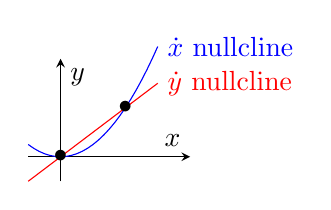
\begin{tikzpicture}
                  \begin{axis}[
                          width=0.3\textwidth,
                          axis lines=middle,
                          no markers,
                          xtick=\empty,
                          ytick=\empty,
                          clip=false,
                          xlabel={$x$},
                          ylabel={$y$},
                          domain=-0.5:1.5,
                          ymin=-0.5, ymax=2,
                          xmin= -0.5, xmax=2,
                          view = {0}{90}
                      ]
                      \addplot[red] {x} node[right] {$\dot y$ nullcline};
                      \addplot[blue] {x^2} node[right] {$\dot x$ nullcline};

                      \node at (0, 0) {$\bullet$};
                      \node at (1, 1) {$\bullet$};

                  \end{axis}
              \end{tikzpicture}
          \end{center}
          \color{black}

    \item Find and classify all equilibria (Hint: use the determinant and the trace).

          \color{red}
          The nullclines give us equilibria at $(0, 0)$ and $(1, 1)$.

          \begin{align*}
              J(x, y) & = \begin{pmatrix}
                              -2x & 1  \\
                              1   & -1
                          \end{pmatrix}                              \\
              J(0, 0) & = \begin{pmatrix}
                              0 & 1  \\
                              1 & -1
                          \end{pmatrix} \implies \begin{cases}
                                                     \det J = -1 \\
                                                     \tr J = -1
                                                 \end{cases} \implies \\
              J(1, 1) & = \begin{pmatrix}
                              -2 & 1  \\
                              1  & -1
                          \end{pmatrix} \implies \begin{cases}
                                                     \det J = 1 \\
                                                     \tr J = -3
                                                 \end{cases}
          \end{align*}

          \color{black}

    \item Sketch the phase portrait.

          \begin{center}
              \color{black}
              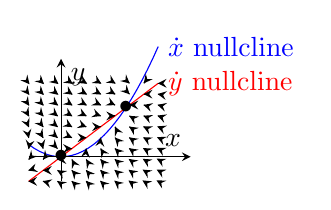
\begin{tikzpicture}
                  \begin{axis}[
                          width=0.3\textwidth,
                          axis lines=middle,
                          no markers,
                          xtick=\empty,
                          ytick=\empty,
                          clip=false,
                          xlabel={$x$},
                          ylabel={$y$},
                          domain=-0.5:1.5,
                          ymin=-0.5, ymax=2,
                          xmin= -0.5, xmax=2,
                          view = {0}{90}
                      ]
                      \addplot[red] {x} node[right] {$\dot y$ nullcline};
                      \addplot[blue] {x^2} node[right] {$\dot x$ nullcline};

                      \addplot3[-stealth, quiver={
                                  u=(-x^2 + y),
                                  v=(x - y),
                                  scale arrows=0.01,
                              }, samples=10] {0};

                      \node at (0, 0) {$\bullet$};
                      \node at (1, 1) {$\bullet$};

                  \end{axis}
              \end{tikzpicture}
          \end{center}

    \item Can this system have any periodic orbits? Support your answer.
\end{enumerate}

\pagebreak

\section{Problem 7}
Find all equilibria and classify their bifurcation points for the differential equation
\begin{align*}
    \dot x & = 1 -(b + 1)x + ax^2y \\
    \dot y & = bx -ax^2y,
\end{align*}
where $a,b > 0$ are strictly positive parameters.

\color{blue}
\[\begin{array}{rl}
        0 & = 1 - bx - x + ax^2y \\
        0 & = bx - ax^2y         \\ \hline
        0 & = 1 - x
    \end{array} \implies x = 1 \implies b = ay \implies (1, b/a)\]
and
\begin{align*}
    J(x, y)   & = \begin{pmatrix}
                      -(b + 1) + 2axy & ax^2  \\
                      b - 2axy        & -ax^2
                  \end{pmatrix}        \\
    J(1, b/a) & = \begin{pmatrix}
                      -(b+1) + 2b & a  \\
                      b - 2b      & -a
                  \end{pmatrix} = \begin{pmatrix}
                                      b - 1 & a  \\
                                      -b    & -a
                                  \end{pmatrix}
\end{align*}

And
\[\begin{cases}
        \det J = -a(b-1) + ab = a > 0 \\
        \tr J = b - 1 - -a
    \end{cases} \implies \text{ saddle}\]


\color{black}


\end{document}
